%!TEX encoding = UTF-8 Unicode
% ================================================================================
\documentclass[
    fontsize=12pt,
    headings=small,
    parskip=half,           % Ersetzt manuelles Setzen von parskip/parindent.
    bibliography=totoc,
    numbers=noenddot,       % Entfernt den letzten Punkt der Kapitelnummern.
    open=any,               % Kapitel kann auf jeder Seite beginnen.
    final                   % Entfernt alle todonotes und den Entwurfstempel.
]{scrreprt}

% ===================================Praeambel==================================
%!TEX encoding = UTF-8 Unicode
%!TEX root = expose.tex

\usepackage[T1]{fontenc}
\usepackage[utf8]{inputenc}
\usepackage{microtype}      % Optimale Randausrichtung und Skalierung.
\usepackage[
    autostyle,
    ]{csquotes}             % Korrekte Anführungszeichen in der Literaturliste.
\usepackage{scrhack}        % Verhindert Warnungen mit älteren Paketen.
\usepackage[
  newcommands
]{ragged2e}                 % Verbesserte \ragged...Befehle
\PassOptionsToPackage{
  hyphens
}{url}                      % Sorgt für URL-Umbrüche in Fußzeilen u. Literatur
% }}}

% Schriftarten {{{
\usepackage{mathptmx}       % Times; modifies the default serif and math fonts
\usepackage[scaled=.92]{helvet}% modifies the sans serif font
\usepackage{courier}        % modifies the monospace font
% }}}

% Biblatex {{{
\usepackage[
    style=alphabetic,
    backend=biber,
    %backref=true
    ]{biblatex}             % Biblatex mit alphabetischem Style und biber.

\addbibresource{\jobname.bib} % Dateiname der bib-Datei.

\DeclareFieldFormat*{title}{
    \mkbibemph{#1}}         % Make titles italics
% }}}

% Dokument- und Texteinstellungen {{{
\usepackage[
    a4paper,
    margin=2.54cm,
    marginparwidth=2.0cm,
    footskip=1.0cm
    ]{geometry}             % Ersetzt 'a4wide'.
\clubpenalty=10000          % Keine Einzelzeile am Beginn eines Absatzes
                            %  (Schusterjungen).
\widowpenalty=10000         % Keine Einzelzeile am Ende eines Absatzes
\displaywidowpenalty=10000  %  (Hurenkinder).
\usepackage{floatrow}       % Zentriert alle Floats
\usepackage{ifdraft}        % Ermöglicht \ifoptionfinal{true}{false}
\pagestyle{plain}           % keine Kopfzeilen
% \sloppy                    % großzügige Formatierungsweise
\deffootnote{1em}{1em}{
  \thefootnotemark.\ }      % Verbessert Layout mehrzeiliger Fußnoten
\renewcommand*{\chapterformat}{% Hübscht Kapitelüberschrift mit senkrechtem 
	\thechapter\enskip%          grauen Balken zwischen Nummer und Text auf
	\textcolor{gray!50}{\rule[-\dp\strutbox]{2pt}{\baselineskip}}\enskip
}
%\setkomafont{disposition}{\normalcolor\bfseries} % Aus der KOMA-Skript-Anleitung: „Mit dieser Änderung verzichten Sie darauf, für alle Gliederungsebenen serifenlose Schrift voreinzustellen“

\makeatletter
\AtBeginDocument{%
    \hypersetup{%
        pdftitle = {\@title},
        pdfauthor  = \@author,
    }
}
\makeatother
% }}}

% Weitere Pakete {{{
\usepackage{graphicx}       % Einfügen von Graphiken.
\usepackage{tabu}           % Einfügen von Tabellen.
\usepackage{multirow}       % Tabellenzeilen zusammenfassen.
\usepackage{multicol}       % Tabellenspalten zusammenfassen.
\usepackage{booktabs}       % Schönere Tabellen (\toprule\midrule\bottomrule).
\usepackage[nocut]{thmbox}  % Theorembox bspw. für Angreifermodell.
\usepackage{amsmath}        % Erweiterte Handhabung mathematischer Formeln.
\usepackage{amssymb}        % Erweiterte mathematische Symbole.
\usepackage{rotating}
\usepackage[
    printonlyused
    ]{acronym}              % Abkürzungsverzeichnis
\usepackage[
    colorinlistoftodos,
    textsize=tiny,          % Notizen und TODOs - mit der todonotes.sty von
    \ifoptionfinal{disable}{}%  Benjamin Kellermann ist das Package "changebar"
    ]{todonotes}            %  bereits integriert.
\usepackage[
    breaklinks,
    hidelinks,
    pdfdisplaydoctitle,
    pdfpagemode = {UseOutlines},
    pdfpagelabels,
    ]{hyperref}             % Sprungmarken im PDF. Lädt das URL-Paket.
    \urlstyle{rm}           % Entfernt die Formattierung von URLs.
%\usepackage{breakurl}
%\def\UrlBreaks{\do\/\do-}
\usepackage{listings}       % Spezielle Umgebung für Quelltextformatierung.
    \lstset{
        language=C,
        breaklines=true,
        breakatwhitespace=true,
        frame=l,            % Linie links: l, doppelt: L
		framerule=2.5pt,    % Dicke der Linie
		rulecolor=\color{gray},% Farbe der Linie
        captionpos=b,
        xleftmargin=6ex,
        tabsize=4,
        numbers=left,
        numberstyle=\ttfamily\footnotesize,
        basicstyle=\ttfamily\footnotesize,
        keywordstyle=\bfseries\color{green!50!black},
        commentstyle=\itshape\color{magenta!90!black},
        identifierstyle=\ttfamily,
        stringstyle=\color{orange!90!black},
        showstringspaces=false,
        }
%\usepackage{filecontents}  % Direktes Einfügen von Dateiinhalt. Wird hier für
                            %  die Verwendung einer .bib-Datei in dieser .tex-
                            %  Datei benötigt.
% }}}


\addbibresource{thesis.bib}

% ===================================Dokument===================================

\begin{document}

\title{On using privacy preseving machine learning for\\decentralized web bot detection}
\author{Matz-Jona Radloff}
% \date{01.01.2015} % Falls ein bestimmtes Datum eingesetzt werden soll, einfach
                    %  diese Zeile aktivieren.


\begin{titlepage}
\begin{center}\Large
	\vfill
    Bachelor Thesis
	\vfill
	\makeatletter
	{\Large\textsf{\textbf{\@title}}\par}
	\makeatother
	\vfill
    submitted by
	\par\bigskip
	\makeatletter
	{\@author} \par
	\makeatother
	Matriculation number 6946325 \par
	Study Program: Computer Science
	\vfill
	\makeatletter
	submitted on {\@date}
	\makeatother
	\vfill
	Supervisor: August See\par
	First reviewer: Prof. Dr. Mathias Fischer \par
	Zweitgutachter: N.N.
\end{center}
\end{titlepage}


\chapter*{Abstract}

Malicious use of automated bots presents an increasing risk to applications in the web. Their detection represents an integral part of modern security system. Existing solutions do either not perform well, are not accessible to many providers due to high cost, or disregard modern privacy standards. This work aims to provide a proof-of-concept for a basic system that incorporates all of the above criterions. It utilizes biometric data in the form of pointer interactions.

\tableofcontents

\chapter{Introduction}

In this work, the term bot is referring to software that is automatically performing HTTP(S) requests with the intent of harming a target or reaching another malicous goal. While this threat is nothing new to the web the attack surface has grown significantly over the past years \cite{BAD_BOT_REPORT2020,BAD_BOT_REPORT2021}. Especially the increased usage of web interfaces in poorly secured IoT devices and the trend to (re-)implement software as web applications is responsible for this.

The usage of bots can have several goals. This thesis primarily focuses on detecting web-based bots that try to access or perform actions on websites. Other and related attack types exist, for example:
DoS attacks aim to overload the target's infrastructure such that it becomes inaccessible for normal use. Carding and Credential stuffing refers to performing payment or login requests to find working credit card numbers and credentials usually obtainend from a data breach. Data scrapers download the website information and can use it for malicious purposes, e.g. damage SEO or violate copyrights. Content spam includes inserting malicious or polluting data on platforms that allow user generated content. Scalping or inventory hoarding of shopping items can artificially raise prices, damage brands, generate false market forces and create a bad customer experience.

Recent studies show that of 2020's internet traffic 25.6\% was fraudulent and automatically generated \cite{BAD_BOT_REPORT2020} \cite{BAD_BOT_REPORT2021}. They also show that both the percentage of bot traffic in general and malicious bot traffic has increased over time.

Most of the above attacks need to trick the webserver and application backends into performing the request as if it had been initiated by a human. Instead of combating the resulting issues separately, bot detection could potentially mitigate many at once.

A complication in this problem space is the, often desired, requirement for non-malicious bots to be granted normal access. A prominent example are scraper bots used by search engines that need to request websites periodically to build their search indices. A common technique to exploit this requirement is trying to emulate known bot signatures from large search engines, e.g. Googlebot \cite{8421894}.

Many website operators tend to use solutions that are easy to integrate. This requires embeding external software which collects user data and sends it to servers of the software vendors. Closed source software does not allow to determine what exactly happens to the user data and website operators open themselves to additional threats in case of a data breach. Depending on the operating countries of both the websites and software vendors, data privacy regulation might also not allow sharing user data at all or require the operator to document the data transfers in a very detailed and legally complicated way. For example, in countries falling under the GDPR \cite{GDPR} a comprehensive data protection documentation is required. Because of the above reasons it is desirable to either employ self-hosted software or use a solution that does not require user data transfers.



\chapter{Requirements and Related Work}

%\section{Proprietary Solutions}
%\url{https://datadome.co/} \\
%\url{https://www.perimeterx.com/products/bot-defender/} \\
%\url{https://www.imperva.com/products/advanced-bot-protection-management/} \\
%\url{https://www.fastly.com/products/cloud-security/bot-protection} \\
%\url{https://www.cloudflare.com/products/bot-management/} \\
%\url{https://developers.google.com/recaptcha/docs/v3} \\
%\url{https://www.hcaptcha.com/} \\

\section{Requirements}

The main requirement of a bot detection system is its performance including being reliable, having a low false positive rate and good execution speed. If these factors are degraded by including other features, this work defines the overall value still lower as without.

Meeting the requirements would be easier if the whole or critical parts of the underlying system were publicly available, preferably as open source.

Other optional challenges are ease of use for the operator and integration into existing solutions.

The most desirable additional requirement is privacy friendliness, the feasibility of which this work aims to show. For this to be met a level of transparency is required in order to comprehend the user data flow. Proprietary solutions needed to be trusted or individual agreements needed to be found.


\section{Related Work}

The paper \cite{LiJi2021} introduces a federated learning approach similar to the goals of this work but differs in the specific use case and implementation. Their system focuses on the detection of IoT (Internet of Things) devices which are easily hacked and turned into zombies. These zombies are commonly used in DDoS (Distributed Denial of Service) attacks which their strategy tries to make not feasible to perform. They also develop their own iterative model averaging based method "gated recurrent unit" (GRU) which is optimized for their specific use case.

Iliou et al. \cite{10.1145/3339252.3339267} present a comparison of different machine learning algorithms and combinations of different attributes used in previous literature. The attributes comprise mostly of request metadata which would be suitible for a privacy-friendly bot detection system, for example the percentage of image requests or the number of total bytes per session. The authors split the bot data in their dataset into simple and advanced bots which is determined by whether the requests have a browser agent name and, in case they do, whether the IPs have shown malicious activity before. Their results show that different sets of attributes are performing best depending on the classification algorithm used. The best performing ones are Random Forest and Multilayer Perceptron although the paper concludes that using an ensemble classifier that averages over all used methods would be more stable. Additionally simple web bots can be detected very easily while detecting advanced bots is significantly harder, with areas under the ROC curve of $1.00$ and $0.64$ respectively. Especially in false positive intolerant use cases the performance of detecting advanced bots is too poor to be used in the real world. The authors conclude that future work would need to incorporate more advanced features which can not be easily simulated by bots.

The work of \cite{PETS2021} outlines the problems and privacy-related concerns really well and tries to solve a very similar problem but focuses on mobile devices. The authors run a pre-trained machine learning model on the user's device. To avoid local changes to the model a cryptographic proof is generated that is verified on a server.

Among others, the works of Shen et al. \cite{6263955} and Antal et al. \cite{9111596} show the viability of using mouse and trackpad actions to verify the authenticity of users.
Shen et al. use a pattern-growth-based mining method which results in false negative and false positive rates of $1.12\%$ and $0.37\%$ respectively.
Antal et al. report $0.92$ and $1$ AUC for the test and training part of the Balabit dataset \cite{BALABIT_CHALLENGE} with their two-class classifier.
Privacy concerns were cited as one the primary challenges of using such a methods in practice. Their good perfomance makes using mouse data a promising method if these concerns could be remedied.

Antal et al.\cite{9111596} and their previous paper\cite{DBLP:journals/corr/abs-1810-04668} segment raw mouse data into mouse actions such as mouse move (MM) or mouse move and a click (point and click, PC). Multiple results can be averaged to increase detection performance. \todo{more info}

Additionally Acien et al. \cite{Acien2020BeCAPTCHAMouseSM} also show the feasibility of using biometric features for bot detection in general and propose new mouse trajectory synthesis methods as well as a GAN-based learning system that can distinguish between humans and bots with $93\%$ accuracy with only one mouse trajectory as input.


\chapter{Method}

\section{Concept}

The thesis explores how biometric data can potentially improve a machine learning system for bot detection. A ML-based system is chosen because methods like federated learning \cite{DBLP:journals/corr/KonecnyMR15} \cite{DBLP:journals/corr/KonecnyMRR16} can be used to transfer learned knowledge of different bot behavior between systems without compromising user privacy in comparison to traditional methods. It consequently allows the incorporation of very sensitive personal data which, this work hypothesizes, will improve the performance.

For comparison a similar system to the proposed architecture of Iliou et al. \cite{10.1145/3339252.3339267} is implemented. The authors propose a machine learning based web bot detection framework which operates on request log data. They also identify which extracted features of the data perform best in this context. Their method was tested on a year's worth of HTTP log data from MK-Lab's public web server\footnote{Multimedia Knowledge and Social Media Analytics Laboratory, \url{https://mklab.iti.gr/}}. The data includes IP addresses, request method, request path, referrers, user agent strings and timestamps.
Iliou et al.'s work is used as the basis for the machine learning system of this thesis because they compared the most promising features that have been proposed over 5 years prior to their publication (2019) and accumulated their findings in concise results.

Mouse, touchpad or touch gestures (pointer data), which are not considered by Iliou et al. \cite{10.1145/3339252.3339267}, supplement the data in this work's approach. This type of data is harder to fake by attackers trying to emulate human behavior and would be classified as sensitive user data. It could not reasonably be used by a third party provider and would require explicit user consent \cite{GDPR}. As this type of data collection would be hard to justify as strictly necessary, it would be best to process the data in an anonymized and indirect way which this method of machine learning provides.

This work hypothesizes that a system using pointer data outperforms the compared to one using request metadata and thus justifes the use of sensitive user data.

It will also be shown that the requirement of good execution speed is met by integrating the trained model into the experiments' websites as representative real-world applications. As the recorded data is aggregated over time per user, each server response includes the current score as a number between 0 and 1. How much of the past data can be used without compromising request performance will additionally be determined.

\section{Datasets}

To realistically match request metadata and user mouse data a dataset is gathered from two websites in a user experiment. This way biases of different datasets are eliminated and the different systems' performances can be directly compared against.

The websites have a basic blog-style structure with different information sections and user registration features. Their web servers log all relevant data to extract the features required for the request data approach while a javascript library records mouse data and sends it to the site's backends for storage.

To verify the proposed system does not overfit to the experiment's limited data, different public data is used to compare against. While no suitible datasets exist that include both request and mouse data, datasets that contain real-world user mouse movement and interaction data are publicly available.

The Balabit Mouse Dynamics Challenge dataset \cite{BALABIT_CHALLENGE} includes a few longer and several shorter sessions which are meant to be used for training and testing respectively.
Antal et. al's dataset \cite{9111596} includes 21 users with around 20-30 sessions each. Their work compares their own dataset against the Balabit and ChaoShen datasets. In their scenario of detecting whether mouse data belongs to a specific user, the former corresponds to better but comparable results.
At the time of publication the referenced ChaoShen dataset is not available anymore.

Antal et. al's dataset is used to validate the transferability of this method because of its better performance and because the other datasets are older and have been used more in other publications.


\section{Machine Learning Model}

Many different machine learning models are suitable for binary classification. Hu et al. \cite{8275816} compare different classifiers in a context where mouse data is used. Random Forest and Multilayer Perceptron (MLP) perform the best.
Iliou et al. \cite{10.1145/3339252.3339267} also show that Random Forest and MLP perform well when using request metadata.

Random Forest\cite{Breiman2001} is a perturb-and-combine technique that uses an ensemble of decision trees with randomized input sample selection and parameters. The randomness has the goal of decreasing the variance and avoid overfitting which are common problems in single decision trees. The final prediction is calculated from the average over all trees. The used implementation's documentation notes that compared to the original publication, their method averages over the probabilistic predictions, instead of only single decisions.\footnote{\url{https://scikit-learn.org/stable/modules/ensemble.html\#random-forests}}

Multilayer Perceptron describes a type of feedforward artificial neural network which connects many perceptron algorithm instances. It is inspired by biological neural networks and has at least three layers (input, hidden, output) which are usually fully connected. By iterating over training data, values for the perceptron's weighted inputs are learned such that the overall system behaves as a classifier or system for regression analysis.

As their performance is comparable in this context and Random Forest's implementation is easier as well as more performant compared to MLP, the former is chosen for this work.

\subsection{Model Parameters}

The most important parameters of the Random Forest algorithm are the number of estimators (i.e. number of decision trees) and the maximum number of randomly selected features per estimator.

Additional parameters include the maximum depth of trees, the minimum number of samples required to split a node in the trees and the minimum number of samples required to be at a leaf node.

An empirical search will determinte the best parameters for this use case.

\subsection{Feature Selection}

Iliou et al. \cite{10.1145/3339252.3339267} ranked the best performing metrics for simple and advanced bots per classification algorithm. For Random Forest, some attributes are not suitible in this theses. For example the authors include a boolean indicating whether a request has a known search engine in their "Referer" header (attribute 14). Because participants are asked to visit the websites directly this attribute is omitted. The websites are otherwise designed such that all of the above attributes are meaningful. The used attributes are listed in the implementation section.

The following selection from Iliou et al.' work \cite{10.1145/3339252.3339267} is used.

\begin{enumerate}
	\item The percentage of HTTP requests that led to an HTTP 4xx code response. (7)
	\item The percentage of HTTP requests that requested a css file. (10)
	\item The percentage of HTTP requests that requested a JavaScript file. (11)
	\item The percentage of HTTP requested URLs that contain the previously requested URL as a subpart. (20)
	\item The total time (in seconds) between the first and the last HTTP request of the session. (21)
	\item Standard deviation of requested pages' depth (i.e. number of ’/’ in URL path).
\end{enumerate}

The mouse data features will consist of the (normalized) $x$- and $y$-coordinates as well as a time value for each mouse event. Additional features will be engineered similar to \cite{DBLP:journals/corr/abs-1810-04668}, including mean, standard deviation, minimum and maximum value of path tangent, horizontal, vertical and overall velocity, acceleration, jerk, angular velocity. Additionally the type of action, length of the movement and time needed to complete the action will be used.

Single mouse data points are grouped based on the following rules: They either end with a click, have a maximum of 50 data points or span a maximum of two seconds. The features are calculated for each group.


\subsection{Classification and Evaluation}

The actual classification is performed by splitting the extracted features into training and test data. The partitions contain 90 and 10 percent of the data, respectively, with each data entry being assigned randomly. The training data also includes the "is bot" label which the model uses to calculate its error while learning. In the testing phase a predicted label is compared to the known value. The fraction of correct over the total number of predictions, i.e. accuracy is used as the primary evaluation metric. Additionally the False Positive Rate (FPR) and False Negative Rate (FNR) are computed which are the fraction of wrong guesses. The False Positive Rate is weighed higher because a prediction that a user is a bot has a qualitatively much greater impact than the opposite case. Plotting one against the other results in a Receiver operating characteristic (ROC) curve. The area below this curve (AUC) is another good metric for comparing results because it provides a single numerical value. When using normalized units, its concrete value represents the probability that the model will perform better when given a randomly selected positive and negative sample.\cite{FAWCETT2006861}


\section{Experiment/Data Collection}

A user experiment was announced to all members of the University of Hamburg to gather a representative dataset for human interactions on websites. The specific goal of the experiment was not directly included in the announcement to avoid any biases as much as possible. To gather all required data a custom website with two different frontend layouts and designs was implemented.

\subsection{Websites}

The basis of both websites is a Flask\footnote{\url{https://flask.palletsprojects.com/}}-based python application. They are deployed behind a nginx reverse proxy web server which exposes them on two public domains. Their structure and content mimic blog-style websites with login and register functionality. They contain a landing page, an about page with additional information about the experiment and this thesis and a contact / imprint page.
On first visit users get presented a dialog asking to confirm the data collection.
After registering or logging in a profile page is accessible where basic user information can be added or edited. The main part of both websites is a blog section containing randomly generated entries which can be viewed on an overview page or on detail pages.\todo{crap formulation}.
All parts give similar opportunity for user input as regular websites including many possible navigation paths and form interaction.

One difficulty of recording both request and mouse data is that the former benefits from having as many requests per interaction as possible while full page reloads would restart the mouse data collection and might lose data. Usually websites would decide between a traditional approach, where URL changes would load a completely new page and fulfill the former requirement, and a SPA (Single Page Application) where only parts of the content are changed dynamically by JavaScript implementations which would allow mouse events to be recorded continuously.

To combine the advantages of both approaches a hybrid system is used that intercepts URL changes, e.g. from clicking a link, preventing the default action and loading the target page through a separate HTTP request. The main content section is then replaced by the newly loaded HTML data. From the backend's point of view at least one request is performed per visited page while mouse data is recorded without any gaps.

All users, logged in or not, are identified by a version 4 UUID which is immediately stored in cookie after accepting the initial dialog prompt. Every data point that is written to the postgresql database gets a reference to the correspoding user and the current date and time.

\subsubsection{Request Metadata}

For the request metadata relevant information of every request is recorded. Flask allows to register functions which are called at specific points in the request lifecycle. For this purpose the \lstinline{after_request} decorator is used which is called right before the handled request is returned.

Bot data is generated by sending requests to the same websites but including an additional query string which details the current bot configuration.

The following data is stored in the database:

\begin{table}[]
\begin{tabular}{|l|l|}
\hline
user uuid & The current user's UUIDv4 \\ \hline
request method & One of \{'GET', 'POST'\}, other request methods are not used \\ \hline
request url & The full request URL including scheme, host, root path, path and query string \\ \hline
request path & The request path \\ \hline
request origin & The host from which the request was sent from \\ \hline
request remote address & The IP address of the client \\ \hline
request referrer & The referer value from the corresponding header field \\ \hline
response content type & The response's body media type \\ \hline
response content length & The response's body size in bytes \\ \hline
response date & The date and time of the response \\ \hline
response status code & The HTTP status code of the response \\ \hline
user type & One of {Bot, Human} \\ \hline
random delays & Whether random delays for bot-generated requests were enabled \\ \hline
advanced & Whether the advanced bot version was used \\ \hline
bot mode & One of \{Request, Mouse\} \\ \hline
data type & One of \{Request, Mouse\} \\ & saved separately because e.g. mouse bots also generate request data \\ \hline

\end{tabular}
\end{table}

\subsubsection{Mouse Data}

All information for the mouse datasets is recorded by a JavaScript library which is deployed as part of a VueJS application. It registers listener functions for the events \lstinline{pointermove, pointerdown, pointerup} on the whole document which are throttled to $30$ events per second. Pointer events are used because they include mouse, touch, pen/stylus and other pointing devices. For every event the following data is recorded:


\begin{table}[]
\begin{tabular}{|l|l|}
\hline
user uuid & The current user's UUIDv4 \\ \hline
type & One of \{'pointermove', 'pointerdown', 'pointerup'\} \\ \hline
position & The pointer's x and y screen coordinate in pixels \\ \hline
document size & The document's width and height in pixels \\ \hline
pointer type & One of \{'mouse', 'pen', 'touch'\} \\ \hline
buttons & What buttons are pressed as a binary encoded integer \\ \hline
dt & The date and time of when the event occurred \\ \hline

\end{tabular}
\end{table}

All events are cached locally in a list which is sent to the backend every two seconds which writes every data point individually to the database. This request is excluded from the request data capture.

\section{Bot Data Generation}

To generate bot data the different variants are implemented by using the selenium-python \cite{SELENIUMPYTHON} library. It is design to run automated actions in a browser environment.


All bots are implemented as a generic python class \lstinline{Bot} which sets up a selenium\cite{SELENIUMPYTHON} webdriver instance and provides wrapper methods for randomly waiting between calls and locating elements. It starts a  browser instance with a specific window size. Firefox is used as the browser backend and 1366x768, 1920x1080 and 2560x1440 are used as the window sizes as these represent very common monitor resolutions.\footnote{\url{https://gs.statcounter.com/screen-resolution-stats/desktop/worldwide}} It also performs an initial request to set the current bot parameters and saves the returned cookie.

The classes \lstinline{RequestBot} and \lstinline{MouseBot} inherit from \lstinline{Bot} and implement methods for the following actions:

\begin{itemize}
	\item Accepting the initial prompt dialog to start the experiment
	\item Visiting the top-level pages \{About, Blog, Contact/Imprint, Login, Register\}
	\item Visiting randomly selected single blog pages with a parameter for how many (default: $10$)
	\item Visiting completely randomly selected pages with a parameter for how many (default: $100$)
	\item Registering an account
	\item Filling in profile data
\end{itemize}

All actions are configued to wait for the target element to be visible and clickable, scrolling it into view, if not. If configured as such, before each action a random delay between $0$ and $2$ seconds is waited for.

\subsection{Request Bot}

The request bot primarily uses selenium's basic \lstinline{click}, \lstinline{back} and \lstinline{send_keys} methods to perform the actions. Barring the random delays it will perform the actions as fast as possible.

\subsection{Mouse Bot}

The mouse bot uses the same Selenium-based methods for locating elements but replaces the basic actions with Selenium's ActionChains which can automate low-level interactions including mouse movements, mouse button actions and keypresses. By default it interpolates linearly between the starting and ending locations of the movement.

The advanced mouse bot uses the PyAutoGUI\footnote{\url{https://pyautogui.readthedocs.io/en/latest/}} library to provide additional interpolation methods. It can also be more easily extended than Selenium.
The library \footnote{\url{https://github.com/AntoinePassemiers/Realistic-Mouse}} builds on top of PyAutoGUI.
\footnote{\url{https://github.com/patrikoss/pyclick}}


\chapter{Implementation}


\section{Feature Extraction}

First, the stored unique users are filtered based on a minimum number of data points (20). In a (multi-threaded) pre-processing step the feature data is queried, loaded and calculated per user and labeled as "human" or "bot".

\subsection{Request Data Features}

The request data is aggregated per user \todo{per user/max 20?} and the feature data is calculated as described in \nameref{machine_learning_model}.

\subsection{Mouse Data Features}

The mouse data is calculated per user and grouped into actions, similar to \cite{}. Each action represents a mouse movement that is either a maximum of $2$ seconds long or ends with a click. It is also ensured that within any action the screen resolution or page scroll position does not change.


The machine learning input features will consist of the (normalized) $x$- and $y$-coordinates as well as a time value for each mouse event. Additional features will be engineered similar to \cite{DBLP:journals/corr/abs-1810-04668}, such as mean, standard deviation, minimum and maximum value of path tangent, horizontal, vertical and overall velocity, acceleration, jerk, angular velocity. Additionally the type of action, length of the movement and time needed to complete the action will be used.
\todo

\subsection{Classifier Implementation}

% The classifier implementation uses a TensorFlow sequential keras model.
The classifier implementation uses the RandomForestClassifier class from the scikit-learn\footnote{\url{https://scikit-learn.org/stable/}} library.



\chapter{Evaluation}

\section{Experiment Data Quality}

The experiment assumed that participants use the provided website frontends which set cookies to map recorded datapoints to specific users. The first website's basic statistics showed that 124867 unique users have been recorded which indicates that an actual bot was used to visit this website which did not execute Javascript and set the cookie correctly. The histogram of the number of datapoints per users confirms that the vast majority of users only map 0-1 datapoints. With the chosen threshold of 2 datapoints per user the experiment resulted in recording 321 and 240 participants respectively. Figure \ref{fig:user_dp_hist} shows the distribution of the number of user (request and mouse) in terms of the number of datapoints.

\begin{figure}[h!]
	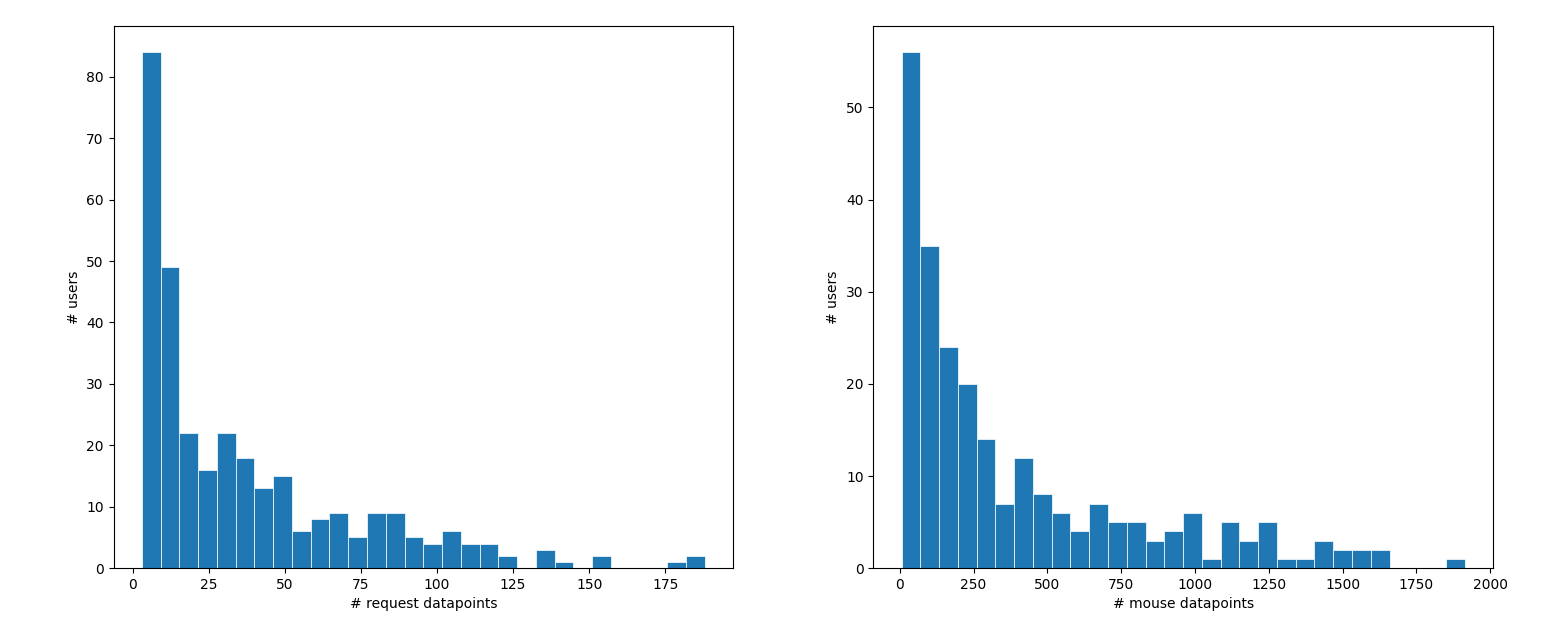
\includegraphics[width=\linewidth]{figures/user_dp_hist.png}
	\caption{Distribution of users in terms of datapoint count}
	\label{fig:user_dp_hist}
\end{figure}



\section{Request Data Performance}

To match the number of users, the same number of bots with variable session length is compared against.

The model's accuracy when only using the request-type data points is $76.60\%$ and $76.92\%$ for the two websites recpectively which indicates that this performance might be a limitation of the model. Their ROC curves \ref{fig:roc_request_both_instances} show that \todo{generate more bot data}.

\begin{figure}[h!]
	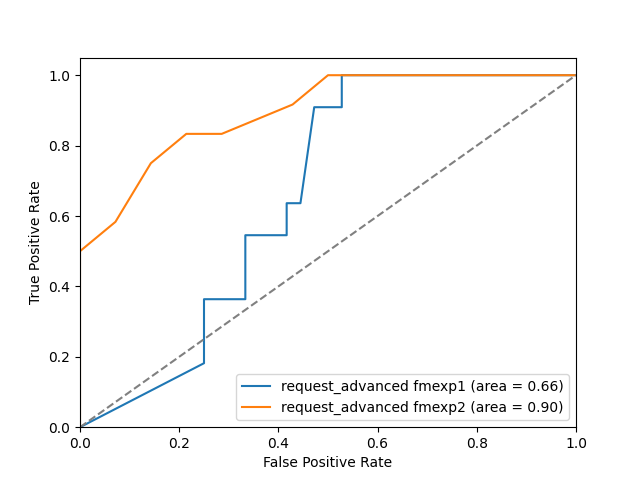
\includegraphics[width=\linewidth]{figures/roc_request_both_instances.png}
	\caption{Distribution of users in terms of datapoint count}
	\label{fig:roc_request_both_instances}
\end{figure}


\section{Mouse Data Performance}

When using mouse data, the classifiers' accuracies are $95.66\%$ and $93.58\%$ which is significantly better compared to using only request data and confirms the hypothesis that bot detection works better when incorporating biometric data. Their ROC curves \ref{fig:roc_mouse_both_instances} show that the requirement for a low False Positive Rate is also met. Their areas under the curve of $0.98$ also show this methods good performance.

\begin{figure}[h!]
	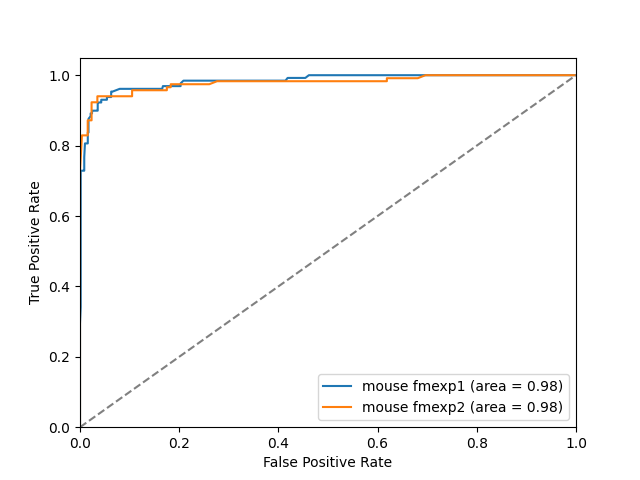
\includegraphics[width=\linewidth]{figures/roc_mouse_both_instances.png}
	\caption{Distribution of users in terms of datapoint count}
	\label{fig:roc_mouse_both_instances}
\end{figure}

\section{Performance on External Dataset}

To compare the performance to different real-world data, Antal et. al's dataset \cite{9111596} is used. Their raw mouse movement and interaction data is preprocessed in the same way as the experiment's data. This results in a much larger test set. For example "User1"'s 31 session files include $2.6M$ raw datapoints which are integrated into $64k$ input vectors.

For comparison the model is trained on data from each instance and both combined. When scoring the model with "User1"'s data as the test set, the model's accuracy increases to $99.11\%$, $99.05\%$ and \todo. For the whole dataset, which resulted in $1.54M$ input vectors, the accuracy dropped to $98.20\%$, $97.94\%$.

\begin{figure}[h!]
	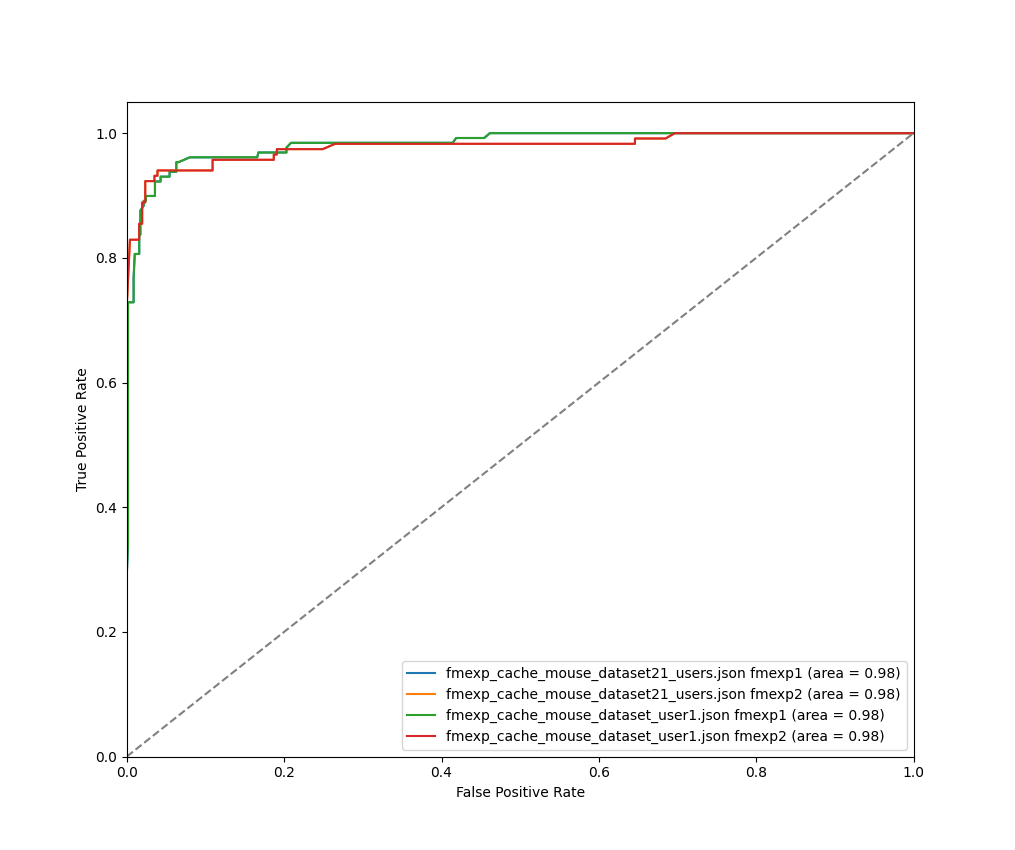
\includegraphics[width=\linewidth]{figures/roc_both_datasets_both_instances.png}
	\caption{ROC curves}
	\label{fig:roc_both_datasets_both_instances}
\end{figure}

\chapter{Discussion}


\chapter{Conclusion}
Bot bad. User data good, nomnom.


\begin{raggedright}
  \printbibliography
\end{raggedright}

% Appendix
\chapter*{Appendix}

\section*{Source Code}

\begin{itemize}
	\item Experiment Websites and Machine Learning Model: Github repository\footnote{\url{https://github.com/timesqueezer/fmexp}} and attached USB drive
	\item Thesis: Github repository\footnote{\url{https://github.com/timesqueezer/uni/thesis}}
\end{itemize}

\end{document}
